\documentclass[11pt]{article}

\usepackage[utf8]{inputenc}
%%\usepackage[T1]{fontenc}
\usepackage{graphicx}
\usepackage[linktocpage=true]{hyperref}

%%Page layout
\usepackage[margin=2.0cm]{geometry}
\usepackage{bookmark}

%%Figures
\usepackage{float}

\usepackage{mathpazo}

%%Font and Numbers
\renewcommand*\rmdefault{dayrom}
\usepackage[T1]{fontenc}
\normalfont
\usepackage{enumitem}

%%Packages for Referrences
\usepackage{url}
\usepackage{etoolbox}
\patchcmd{\thebibliography}{\section*{\refname}}{}{}{}
\patchcmd{\thebibliography}{\addcontentsline{toc}{section}{\refname}}{}{}{}

%%Group Comments
\usepackage{verbatim}

\begin{document}
\renewcommand{\familydefault}{\sfdefault}
\begin{titlepage}
	\newcommand{\HRule}{\rule{\linewidth}{0.5mm}}
	\begin{center}
		            
		\textsc{\LARGE Alabama Liquid Snake}\\[0.8cm]
		\textsc{\Large University of Pretoria}\\[0.5cm]
		\textsc{\large Epi-Use}\\[0.5cm]
		    
		\HRule\\[0.4cm]
		    	
		{\huge\bfseries Botic - Privacy aware chatbot}\\[0.2cm]
		    	
		{\huge System Requirements Specification}\\[0.2cm]
		
		\HRule\\[0.5cm]
		
		\textsc{Justin Grenfell} - u16028440 \\[0cm]
		\textsc{Peter Msimanga} - u13042352 \\[0cm]
		\textsc{Alicia Mulder} - u14283124 \\[0cm]
		\textsc{Kyle Gaunt} - u15330967 \\[0cm]
		\textsc{Lesego Mabe} - u15055214 \\[0cm]
		    
	\end{center}
\end{titlepage}
\tableofcontents
\newpage
\section{Introduction}
\subsection{Purpose}
The purpose of this document is to present a detailed description of Botic- the privacy aware chatbot. It will explain in good detail the purpose and the features of the system, the interfaces of the system, what the system will do, the constraints under which it must operate and also how the system will react to user and external stimuli. This document is intended for the stakeholders, that is the COS 301 staff and lectures as well as the CS department lectures and our client EPI USE Labs-- represented by Mrs. Jhani Coetzee and Mr. Tiaan Scheepers, and the developers, Alabama Liquid Snake, of the system and will be proposed to all of our stakeholders for their approval.

\subsection{Background}
A crucial part of any business in today's economic climate is customer service. Those companies that are willing to go the extra mile for their customers are seen as being a cut above the rest. With superior customer service, a company can not only bring in new clients who want an experience that seems to cater to them as an individual, but also successfully retain existing clients by dealing with their issues efficiently and effectively.\par
In order to do so, there needs to be a system that can record customer feedback and act on it in as soon as possible. In the past, this has been achieved by employing a large number of people around the clock that sat and waited for queries, handled them and sent back the results.\par

While this works, it is not only inefficient (different employees may respond better or worse than others, employees may not follow protocols, mistakes may be made regularly) but financially costly as well. On top of that, when dealing accounts and queries, customers may inadvertently divulge private information that is not applicable to their case, but may leave them vulnerable should that information become public knowledge.\par

What if one central system could seamlessly record, interpret and act on the requests of multiple users 24/7 and prevent them from transmitting sensitive data unless absolutely necessary?\par

\subsection{Scope}
\textbf{Botic} is the solution! One system that can not only record user queries, but sanitize their content by filtering out any "data risks" and act on the provided information, returning the appropriate response. Trained on historical data, the system uses artificial intelligence to analyze requests and act accordingly. It scrapes all data before transmission to ensure that no sensitive information is sent to or from the client without clearance from the sender.\par

Should the system be unable to find a suitable response, the request will be handed off to a customer support representative who will then deal with the request. Once that case has been handled, the system will have learned how to deal with future requests of that type and will be able to return a response based on this learning. This will ensure a high level of efficacy for the system as a whole.\par

%Botic will be the front-line for any company that provides customer service feedback facilities or services. The system will reduce the need for a large number of employees for a problem that can be solved using artificial intelligence. It will also improve efficiency and precision when dealing with issues and, due to its constantly learning nature, will become more accurate and able to handle more complex situations as time goes on.

\subsection{UML Domain Model}

\begin{figure}[H]
	\centering
	\hspace*{-1.7cm}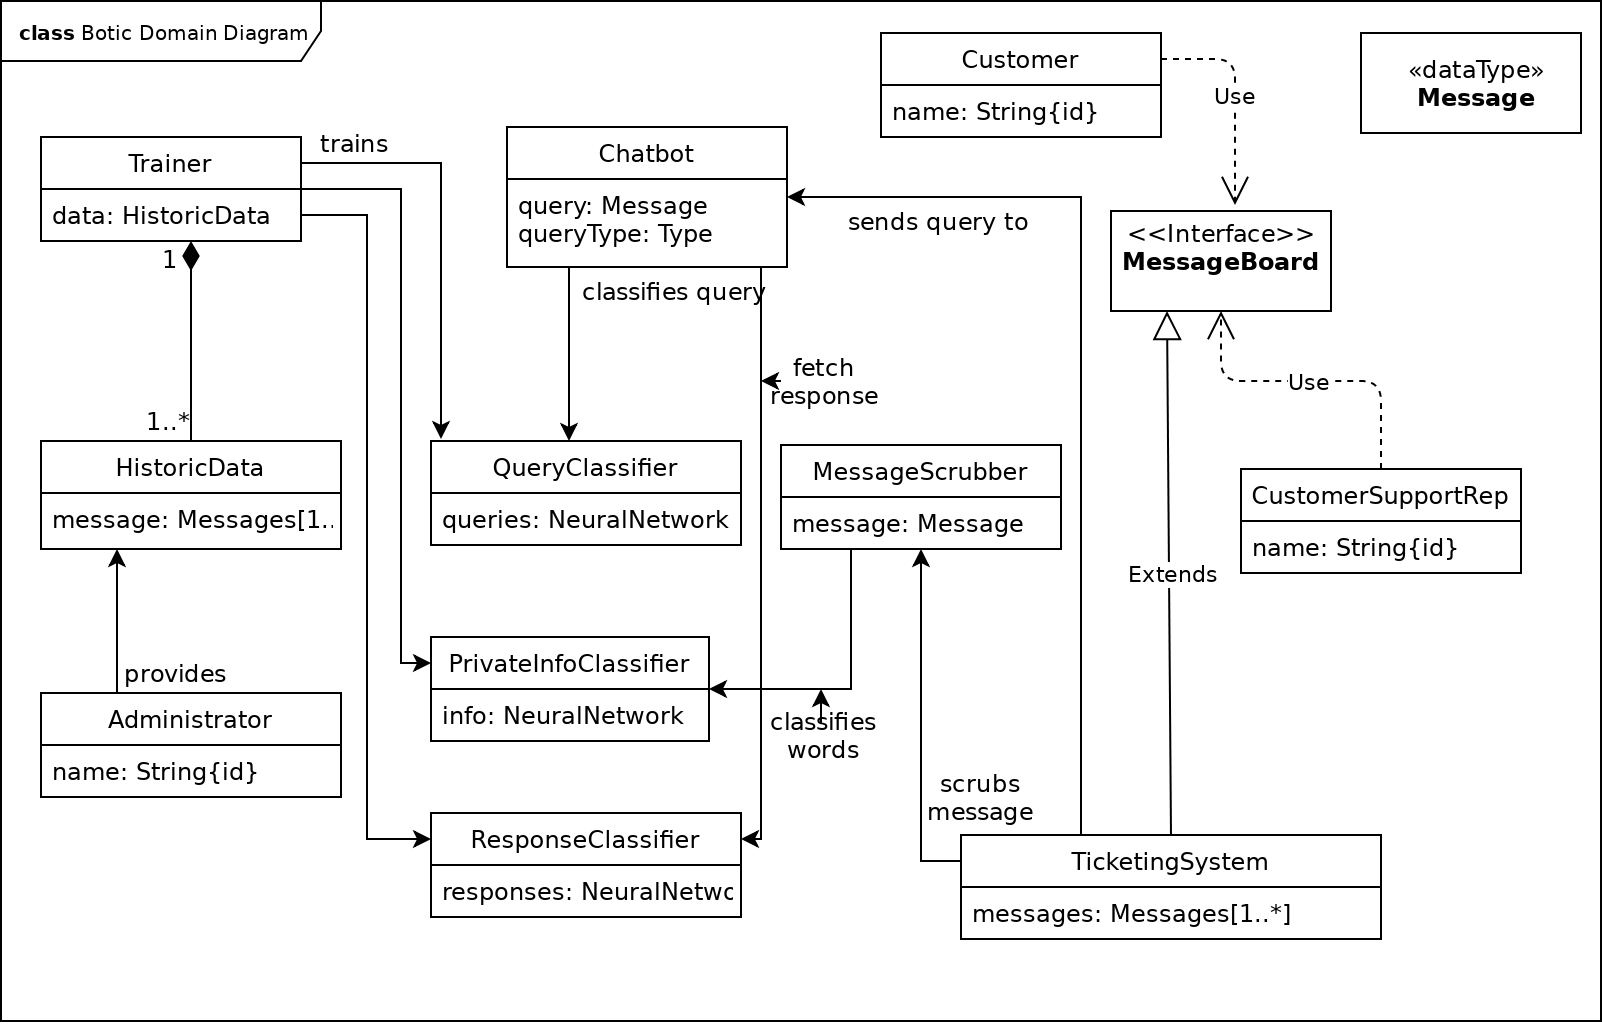
\includegraphics[width=1.2\textwidth]{../../images/Botic_Domain_Diagram.png}
	\caption{UML Domain Model of the Botic System}
\end{figure}

\subsection{Definitions, acronyms, and abbreviations}

\begin{tabular}{ |p{2cm}|p{14.7cm}| }
	\hline
	Chatbot              & A program that is designed to simulate a conversation as if it were a human, in order to assist one who queries with some task or inquiry. In the context of this project, the chatbot will be used to assit customers in a ticket system (customer service system).                                                                                                                                                     \\
	\hline
	AI                   & Artificial Intelligence;  this refers to programmed intelligence, or rather, intelligence that is demostrated by computers usually to mimick human intelligence in some specific area or even in general terms.                                                                                                                                                                                                          \\
	\hline
	Historic Data        & Data that is collected and stored over some considerable period of it time, especially, in the context of this project, with the purpose of being used to train a chatbot.                                                                                                                                                                                                                                               \\
	\hline
	POPI Act             & Protection of Personal Information Act; an South African piece of legislature aimed at protecting the right of its citizens to privacy, especially in the Internet and its periphery. It aims to "provide for the rights of persons regarding unsolicited electronic communications and automated decision making; to regulate the flow of personal information access the borders of the Republic."\cite{Legislature:1} \\
	\hline
	Ticket System        & An online platform, used by a business, made for processing customer queries and issues on products, services and the like.                                                                                                                                                                                                                                                                                              \\
	\hline
	Personal Information & Sensative and identifying information; the likes of which permission should be asked before sharing or processing.                                                                                                                                                                                                                                                                                                       \\
	\hline
	CS                   & Computer Science, as in the academic discipline of Computer Science.                                                                                                                                                                                                                                                                                                                                                     \\
	\hline
	Scrub                & Detect private information and highlight it according to severity.                                                                                                                                                                                                                                                                                                                                                       \\
	\hline
	SPA                  & Single Page Application; a web application that dynamically changes a signle page to display all of its contents.                                                                                                                                                                                                                                                                                                        \\
	\hline
	Heroku               & Deployment platform.                                                                                                                                                                                                                                                                                                                                                                                                     \\
	\hline
	Docker               & Containerization platform*.                                                                                                                                                                                                                                                                                                                                                                                              \\
	\hline
	Auth0		    &Authorization server; third party software/service; provides authorization and authentication as a service.*
\\
	\hline
\end{tabular}

\subsection{Overview of Document}
The next chapter, the Overall Description section, of this document gives an overview of the functionality of the project. It describes the 'informal' requirements and is used to establish a context for technical requirements specification in the next chapter.\par
The third chapter, the Requirement Specification section, of this document is written especially for the developers and describes in terns the details of the functionality of the product.\par
Both sections of the document describe the same software product in its entirety, but are intended for different audiences and thus use different languages, but seeing as virtually everyone reading this document has a CS background, the main focus ought to be the third section and it is given priority as a result.\par
This document is structured according to the IEEE 830-1998 SRS Standard\cite{Standard:1}, as recommended by:\cite{Book:1}.

\section{Overall Description}
\subsection{Product Perspective}
 
This system was originally meant to be used in an already existing customer support ticketing system, or ticket system in short. This is to say that the ticketbot- or rather, chatbot, was meant to interface with the ticket system and also be trained with the ticket system's historic data without the risk of exposing customer personal information.\par

This is system is meant to process a ticket system's messages or tickets, let the users know if they are exposing personal information, and respond intelligently to the messages otherwise divert the queries to a client representative if no sufficient response can be found.\par

However, for the purposes of this project, we will use a simple SPA to mimick the ticketing system.

\subsubsection{System Interfaces}

The deployment diagram for the Botic system:

%The ticket system interfaces with the message scrubber component by communicating to through the message scrubber's API endpoint. The ticket system sends individual words to the message scrubber which returns the severity of word-- the severity is meant to indicate the critical nature of the information revealed e.g. a password can be given the highest severity. This is done whilst the user is typing their message, and the words are highlighted accordingly in their parent field.\par

%The ticket system also interfaces with the chatbot component by communicating through its API endpoint as well. This is when the ticket system sends scrubbed information to the chatbot to gather a response. Once a call is made, the ticket system is sent a reponse through the same API endpoint it called.

\begin{figure}[H]
	\centering
	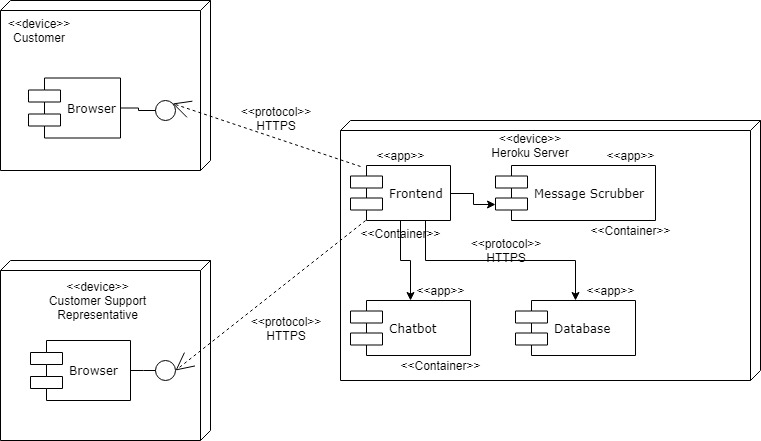
\includegraphics[width=1.0\textwidth]{../../images/Botic_Deployment_Diagram.jpg}
	\caption{UML Deployment Diagram}
\end{figure}

\subsubsection{User Interfaces}

The user interface, which is ultimately the chatbot ticket interface, is meant to be a SPA-- Single Page Application. This should be made available online in a manner that supports all major web browsers.

%Discuss how the user interface will actually interface with the Chatbot API and what kind of API we intend to make


\subsubsection{Hardware Interfaces}

Each subsystem will be containerized into a Docker container, which in and of themselves use Linux 64-bit architecture. 
Ports will be mapped to port 80; this is the standard port for API's and is the port that is exposed on our deployment platform, Heroku.
%%Place the Portmapping Diagram Here, and the Docker container one as well

%%\subsubsection{Software Interfaces}
%%Include snapshots of the packages used in the frontend's packages.json, and go on like that with each subsystem, including
%%specifying how all those subsystems interacted with each other.

%%\subsubsection{Communications Interfaces}
%% SSL, HTTP, et cetera

%%\subsubsection{Memory Constraints} characteristics and limits on primary and secondary memory
%%\subsubsection{Operations} mention backup and recovery operations et cetera
%%\subsubsection{Site Adaptation Requirements} mention dev and production modes

\subsection{Product Functions}%%Functional Requirements;

The Botic system consists of the frontend, AI backend which includes the chatbot API, message scrubber API, the classifier API and their neural networks. The frontend is a Single Page Application which houses the main user interface of the system. The Chatbot API is responsible for recieving messages and returning responses.\par

The Message Scrubber API checks whether or not information provided to it is private and if so, determines the severity of it. The neural networks are trained using Machine Learning and provide the system with its intelligences-privacy classification, responses to queries and queries classification.

%%Use a component diagram to illustrate this point
%%Below this you should have use case diagrams and block diagrams for the architecture
\subsubsection{Authentication}

This subsystem is to be responsible for the authentication and the authorization of customers and customer representatives. This involves the creation and update of user profiles of the mentioned roles. Auth0 will be used as an Authorization server and will be configured to make us of the OAuth 2.0 authorization framework in order to provide us with enough flexibility to create different grants/permissions to easily authorize different users for different activities in the system.

\begin{figure}[H]
	\centering
	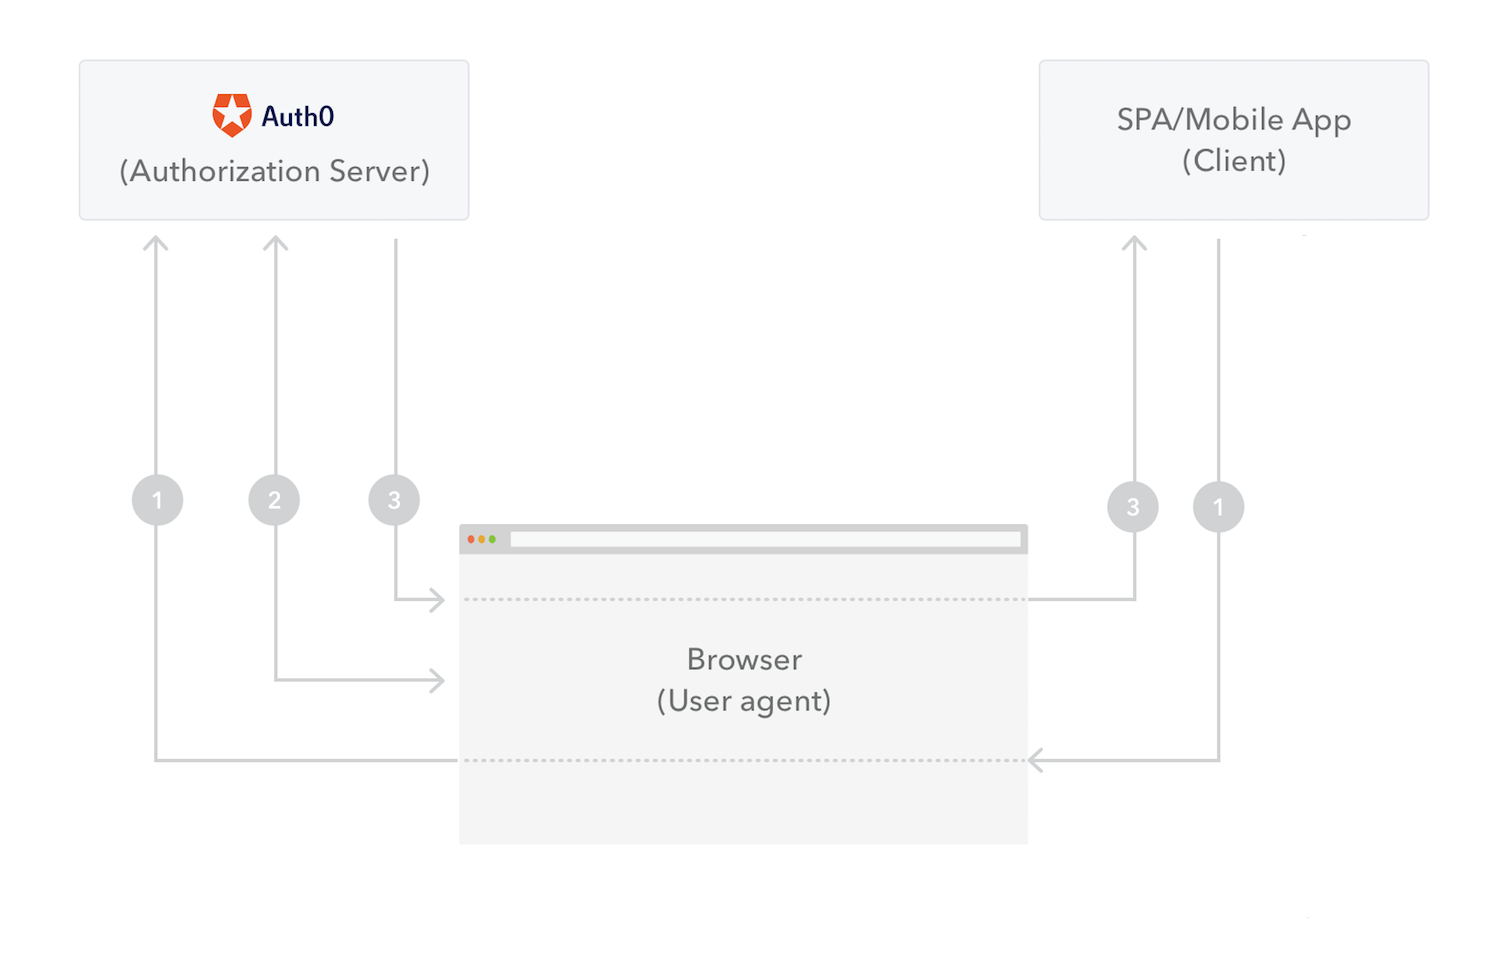
\includegraphics[width=1.0\textwidth]{../../images/implicit-grant.png}
	\caption{Auth0 Solution Diagram\cite{Website:1}}
\end{figure}

\begin{enumerate}
	\item The frontend initiates the flow when the user clicks on the sign in button and redirects the browser to the Auth0 			/authroze endpoint so that the user can be authenticated.
	\item Auth0 then authenticates the user. If the user is using one of the supported social logins, they will be shown a 			consent page where there are permissions, which will be given to our system- Botic, that a listed and they would have to 		give their consent for Botic, through Auth0, to use.
	\item Auth0 then redirects to Botic with an Access Token in the hash fragment of the URI, which the authentication 			module consumes. The happens because Auth0 calls an endpoint on the Botic fronend which processes the token from the 	URI. Botic can now extract the token, and the user is logged in.\cite{Website:1}
\end{enumerate}

\subsubsection{Information Scraper}

\begin{figure}[H]
	\centering
	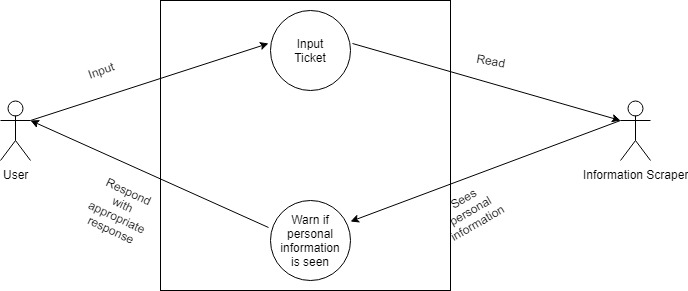
\includegraphics[width=1.0\textwidth]{../../images/Information_Scraper_UCD.jpg}
	\caption{UML Use Case of the Information Scraper}
\end{figure}

The Information Scraper, or Message Scrubber, is a subsystem that is responsible for identifying personally identifying information as the user types in their query. It uses the PrivateInfoClassifier to classify words given to it and to produce a severity index. It is called by an interface that is implemented as an Angular service in the Botic frontend. The API itself is implemented in Python and served using gunicorn. It is containerized using Docker to make it more portable, and also to make it possible to run it and other subsystems in the same infrastructure without much difficulty.

\subsubsection{Chatbot/Ticketbot}

\begin{figure}[H]
	\centering
	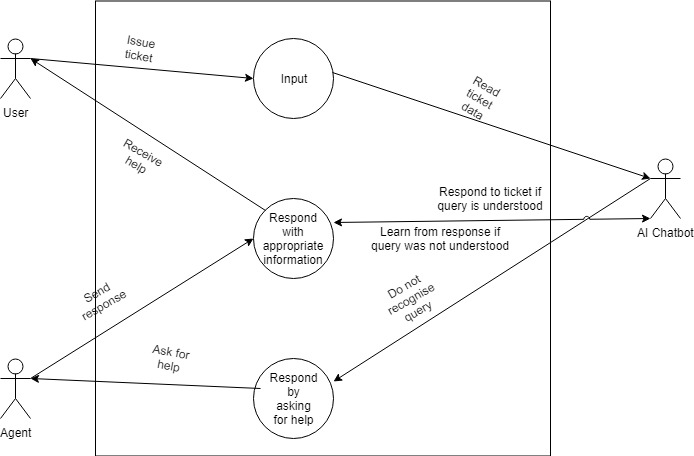
\includegraphics[width=1.0\textwidth]{../../images/AI_Chatbot_UCD.jpg}
	\caption{UML Use Case of the Chatbot}
\end{figure}

The Chatbot or 'Ticketbot' is the subsystem that is responsible for taking in customer queries and answering those queries. The Chatbot consults a QueryClassifier with a query to classify it i.e. whether it is a password, configuration, or other query for example. The classification and the query are then used to find the best response for the query using a neural network of responses, which was initially trained using historical data. The Chatbot is implemented using Nodejs and it is also containerized, for the same reasons as the previous subsystem.

\subsubsection{AI Training}

\begin{figure}[H]
	\centering
	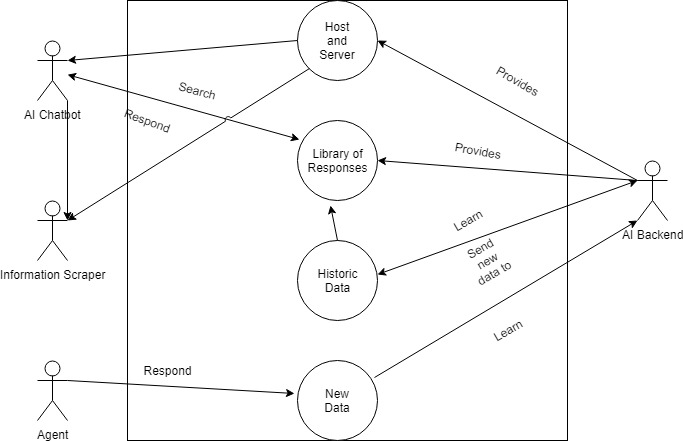
\includegraphics[width=1.0\textwidth]{../../images/AI_Backend_UCD.jpg}
	\caption{UML Use Case of the AI Backend}
\end{figure}

The AI Training subsystem is responsible for training the PrivateInfoClassifier, the QueryClassifier and the Responses neural networks. This is done using historic data which belongs to the ticketing system.

\subsubsection{Database Manager}

This subsystem is responsible for managing persistance in the system. It is called when data needs to be stored, updated, and deleted. Each endpoint will require that the subsystem calling it, identify itself. We intend to have this API secured using JSON Web Tokens. It will be implemented using Java, which when correctly uses, tends to outperform Nodejs is speed\cite{Website:2}  and is a much more rebust language than that of NodeJs's JavaScript\cite{Website:2}. This language choice is also made with consideration to the data analytics what will come about when analyzing and processing logs and their data.
%%It's also much easier to translate knowledge we learnt in COS226 for concurrency usage, than learn to do it with another
%%language due to time constraints. All team members know how to implement concurrency using Java.
%%Also, in terms of maintainability, using Java over time will result in a much faster and robust system.

\subsection{User Characteristics}

\subsubsection{Customer}
The customer will be submitting information to the system in order to deal with account related queries and, in doing so, may unintentionally submit private/sensitive information that could lead to a breach of confidentiality. Any information sent through by the customer will be sanitized by the system and cleaned up before it is transmitted.

\subsubsection{Customer Support Representative}
This user will be notified when the automated system is unable to interpret the customer's request and said request will be forwarded. The user will have the ability to respond with the result, whereby the system will sanitize the data once more and send it through to the customer.

\subsubsection{Administrator}
The system administrator is a super user who will be able to manage the system as well as register customers and customer support representative. The administrator will be able to feed the chatbot historic interactions so that it can be trained with the data to improve the correctness of response generation.

Users with Administrator credentials will have the ability to change the settings and operational preferences of the program to better suit the needs of its company's requirements. Admin will have control over the program as a whole including access control, privacy preferences and overall system operation.

%%\subsection{Constraints}
%%\subsection{Assumptions and Dependencies}
\section{Specific Requirements}
%\subsection{External Interfaces}

\subsection{Functional Requirements} %used to be \subsection{Function}

Requirements are labelled with "R" and constraints with "C."
	
\subsubsection{User Interface}
\begin{itemize}
  \item[] R1.1 The system must allow a customer to enter a query and click on a button to send it.
  \item[] R1.2 The system must warn a customer of personal information included in a query.
  \item[] R2.2 The system must be able to highlight personally identifying information according to severity index.
  \item[] R3.3.2.2 The system must be able to highlight personally identifying information according to severity index.
  \item[] R3.3.2.3 The system must be able to warn the client representative if they have entered identifying information.
  \item[] R4.1 The system must allow customers to thumbs up a query response.
  \item[] R4.2 The system must allow customers to thumbs down a query response.
  \item[] R5 The system must allow queries to be sent to customer support representatives if not answered satisfactorily.
  \item[] C1 The system must use an Angular Single Page Application for the user interface.
\end{itemize}
%%\subsubsection{UI}

\subsubsection{Information Scraper}
\begin{itemize}
  \item[] R2.1 The system must be able to attach a severity to the personally identifying information.
  \item[] R3.1 The system must scrape its customer query responses for personal information.
  \item[] R3.3.2.1 The system must be able to identify personal information in a customer representative's response. 
  \item[] C3.1 The system must use word2vec for identifying personal information in customer queries.
  \item[] C5.2 The system must determine if the response contains personally identifying information.
\end{itemize}

\subsubsection{Query Classification}
\begin{itemize}
  \item[] R3.2 The system must be able to classify the user queries.
  \item[] C3.2 The system must use word2vec for classifying customer queries.
\end{itemize}

\subsubsection{Response Generation}
\begin{itemize}
  \item[] R3.3.1 The system must generate a response if it certain that it can.
  \item[] C5.1 The system must generate an automated response based on the query classification.
\end{itemize}

\subsubsection{Chatbot}
\begin{itemize}
  \item[] R1.3 The system must be able to recieve customer queries.
  \item[] R3.3.2 The system must be able to send the query to a customer support representative if it cannot obtain an appropriate response.
  \item[] R3.4 The system must be able to send a query response back to a customer.
  \item[] R4.3 The system must be able to recieve customer feedback.
  \item[] R5 The system must allow queries to be sent to customer support representatives if not answered satisfactorily.
  \item[] R8 The system must interface with the currently existing ticket system.
  \item[] C2 The system must provide an API for the SPA to interact with.
\end{itemize}

\subsubsection{Chatbot Trainer}
\begin{itemize}
  \item[] R6.1 The system must store previous customer interactions with positive feedback.
  \item[] R7 The system must must be trained with previous customer queries and responses.
  \item[] C4 The system must use Machine Learning or Deep Neural Networks in order to be trained with previous customer queries and responses.
\end{itemize}

\subsubsection{Data Persistence}
\begin{itemize}
  \item[] R9.1 The system must scrape customer interation data for personal information before storing.
\end{itemize}

%\subsection{Performance Requirements}
%\subsection{Design Constraints}
%\subsubsection{Standards Compliance}

\subsection{Organizing the Specific Requirements}

%%\subsubsection{System Mode}
%%\subsubsection{User Class}
%%\subsubsection{Objects}
%%\subsubsection{Feature}
%%\subsubsection{Stimulus}
%%\subsubsection{Response}
%%\subsubsection{Functional Hierarchy}


\subsubsection{Traceability Matrix}
\begin{center}
	\hspace*{-1.3cm}\begin{tabular}{|c|c|c|c|c|c|c|c|}
	\hline
	R & UI & Info Scraper & Query Classification & Resp Generation & Chatbot & Chatbot Trainer & Data Persistence \\
	\hline
	R1.1 & X & & & & & & \\
	\hline
	R1.2 & X & & & & & & \\
	\hline
	R1.3 & & & & X & & & \\
	\hline
	R2.1 & & X & & & & & \\
	\hline
	R2.2 & X & & & & & & \\
	\hline
	R3.1 & & X & & & & & \\
	\hline
	R3.2 & & & X & & & & \\
	\hline
	R3.3.1 & & & & X & & & \\
	\hline
	R3.3.2 & & & & & X & & \\
	\hline
	R3.3.2.1 & & X & & & & & \\
	\hline
	R3.3.2.2 & X & & & & & & \\
	\hline
	R3.3.2.3 & X & & & & & & \\
	\hline
	R3.4 & & & & & X & & \\
	\hline
	R4.1 & X & & & & & & \\
	\hline
	R4.2 & X & & & & & & \\
	\hline
	R4.3 & X & & & & & & \\
	\hline
	R5 & X & & & & X & & \\
	\hline
	R6.1 & & & & & & X & \\
	\hline
	R7 & & & & & & X & \\
	\hline
	R8 & & & & & X & & \\
	\hline
	R9.1 & & & & & & & X \\
	\hline
	C1 & X & & & & & & \\
	\hline
	C2 & & & & & X & & \\
	\hline
	C3.1 & X & & & & & & \\
	\hline
	C3.2 & & & X & & & & \\
	\hline
	C4 & & & & & & X & \\
	\hline
	C5.1 & & & & X & & & \\
	\hline
	C5.2 & & X & & & & & \\
	\hline
	\end{tabular}
\end{center}

Key: UI = User Interface, Info Scraper = Information Scraper, Resp Generation =  Response Generation.

\subsection{Software System Attributes}%%Non-Functional Requirements (limited to 6)

The non-functional requirements below will be listed by priority.

\subsubsection{Availability}
\begin{enumerate}[label=R1.\arabic*.]
	\item The system must have high availability to handle customer queries.
	\begin{enumerate}[label*=\arabic*.]
		\item The system should be available at least 99 percent of the time.
	\end{enumerate}
	\item The system must ensure that errors that occur throughout the system are handled appropriately and provide sufficient
information.
	\begin{enumerate}[label*=\arabic*.]
		\item The system must provide error messages when errors occur.
		\item The system must ensure to keep a traces that show what led to errors.
	\end{enumerate}
	\item The system must ensure that errors are localized and that their effect is minimized throughout the system.
\end{enumerate}

%Perhaps you should include a CIA triad and AAA information set and some figures. 
\subsubsection{Security}
\begin{enumerate}[label=R1.\arabic*.]
	\item The system must be able to authenticate users and authorize them to access system features.
	\begin{enumerate}[label*=\arabic*.]
		\item The system must be able to identify and authenticate customers.
		\item The system must be able to identify and authenticate customer support representatives.
		\item The system must be able to deny users who haven't been authenticated to access system features
	\end{enumerate}
	\item The system must be able to allow new users to register for user profiles for authentication.
	\item The system must be able to allow users to update their password.
	\item The system must ensure that confidentiality of customer and customer support representative interactions are ensured and maintained across the system.
	\begin{enumerate}[label*=\arabic*.]
		\item The system must ensure that customers can interact with the system in a secured manner.
		\item The system must ensure that customer queries are sent in a secured manner.
		\item The system must ensure that customer support representatives care interact with the system in a secured manner.
		\item The system must ensure that customer support representative response are sent in a secured manner.
		\item The system must ensure that all queries and responses are processed in a secured manner.
	\end{enumerate}
	\item The system must ensure that information disclosed during error management is not revealing of internal architecture, design, and configuration information.
\end{enumerate}

\subsubsection{Reliability}
\begin{enumerate}[label=R1.\arabic*.]
	\item The system must ensure that responses to customer queries are done in a reliable manner.
	\begin{enumerate}[label*=\arabic*.]
		\item The system must ensure that customer support representative are authorized to respond to customer queries.
		\item The system must ensure that queries are responses sent throughout the system are complete and consistent.
	\end{enumerate}
	\item The system must ensure that it is at least 80 percent certain that an autogenerated response is correct before responding to a query.
\end{enumerate}

%These are emergent properties that really relly on the performance of multiple if not all of the components of the system.
\subsubsection{Performance}
\begin{enumerate}[label=R1.\arabic*.]
	\item The system must ensure that personal information is highlighted according to severity in real-time.
	\begin{enumerate}[label*=\arabic*.]
		\item The system must ensure that a severity of a word is recieved within a second of it being typed.
		\item The system must ensure that a word or set of words containing personal information are highlighted in less than a second after recieving the severity.
	\end{enumerate}
\end{enumerate}

%Check this out as well
\subsubsection{Scalability}
\begin{enumerate}
	\item The system should be able to scale appropriately to accommodate additional/growing customer queries, especially during peak work hours; it would be useful if the resources scaled down as well during “off peak” hours.
	\item We have chosen to deploy our system to Docker, it is used in part to allow for efficient and easy scaling.% More resources can be allocated to our system dynamically - on demand.
\end{enumerate}

%Need to check this out
\subsubsection{Maintainability}
\begin{enumerate}
	\item The system structure will be modular to adhere to the concept of low coupling and high cohesion. This would help to make it maintainable since updated systems result in localized changes instead of changes everywhere throughout the system.
	\item We will create a coding standards document which we will also adhere to throughout the system in order to increase readability.
\end{enumerate}

%%The following three subsections are not non-functional requirements.
%\subsubsection{Durability}
%\begin{enumerate}
%	\item The system should be able to train by itself based on responses given by a representative without requiring the help of a developer, therefore maintenance and repair to the system should be limited only to updates to the front-end.
%\end{enumerate}

%\subsubsection{Privacy}
%\begin{enumerate}
%	\item The system should be able to identify personal information that was given by the user, and depending on the severity index, warn a user that personal information was sent.
%\end{enumerate}

%\subsubsection{Usability}
%\begin{enumerate}
%	\item The system should be easy to use and understand by any user using the system.  The system should also make it clear what it is being used for so that the user would not question on what to do.
%\end{enumerate}

%These things are not actually constraints. They ought to be removed as well.
\subsection{Challenges}
\begin{enumerate}
	\item Being able to understand what the user is asking even if they use ‘slang’ abbreviations.  For example, using “R U” instead of “are you”.
	\item Not being able to respond adequately to a new user query due to limited or insufficient  training.
	\item Time it would take for a representative to get back to a user if the bot does not know what to respond.
	\item Being prepared for unexpected inputs.
	\item Understanding who the users are, where they are coming from and what they talked about in the past without being able to store/capture and train on data related to specific user data.
	\item Context sensitivity: Handling the users’ possible propensity to change topics in the middle of an interaction which could lead to a possible breakdown in communication (the risk of which is also possible if the AI chooses the wrong context from an ambiguous line of 	conversation).
	\item Ability to determine intent, especially when what is said does not quite match what is meant. (Natural language processing).  Examples:
	\begin{enumerate}
		\item Misused phrases
		\item Intonation
		\item Double meanings
		\item Passive aggression
		\item Poor pronunciation
		\item Speech impairments
		\item Slang
		\item Non-native speakers
	\end{enumerate}
	\item Users requesting multiple tasks and the chatbot being able to respond to those multiple queries.
\end{enumerate}

\subsection{Technology Decisions}
\subsubsection{Technologies}
\begin{enumerate}
	\item Angular
	\item Fasttext
	\item Docker
	\item TravisCI
	\item NodeJS
	\item Python
	\item Git
	\item Gitkraken
\end{enumerate}
\subsubsection{Justifications}
\begin{enumerate}
	\item Angular: A highly portable framework that allows for rapid prototyping, instancing and general development of highly modular, portable applications and components thereof. Chosen because it was specified for by the client but supported by us because of the large amount of support the framework has, being built on nodejs and javascript as a whole. We as a team enjoy the benefits of wide-sweeping platform support.
	\item FastText: An open source library that allows users and developers to create and use text classifiers and text representation. This is the main interface that we are using to train our AI chatbot to recognise the existence of personal information in a given string as well as recognise the type of query that the user is entering for the purposes of giving a suitable response.
	\item Docker: A main goal for this project is to be portable across server implementations and client configurations. Hence the use of web technologies. To solve the server implementations docker provides invaluable aid in the form of containers that can house our backend systems without reck or concern for specific idiosyncrasies across azure, ubuntu and other services. 
	\item TravisCI: Travis is a powerful service that we use to stage integration for our projects. The industry has moved to a standard wherein constant integration, deployment and updating have become the expected norm. To this end, Travis provides tools to integrate new builds on the fly.
	\item NodeJS: Fast server-side javascript by way of Google Chrome’s runtime implementation is exactly what we need to create a networked application such as this. Because Angular is built on Nodejs, the backwards compatibility with existing Nodejs packages is invaluable to us as they mean that we do not have to implement any functionality that hasn’t already been considered to be a solved problem.
	\item Git, GitHub, ZenHub and GitKraken: Git is an industry standard tool for version control so it is obvious that we would use it. Furthermore, because of its ubiquity, git integrates with a large number of tools that make development, version control and project management easier or larger teams.
	\begin{enumerate}
		\item Github: Hosts out code online to trigger hooks in other pieces of software (i.e. travis, docker, heroku) for the purposes of building, deployment and integration. It also keeps track of the versions and iterations of the code that each member of the group has created.
		\item ZenHub: This combines the Kanban method of organising seen in applications like trello and the code integrated version control of github to create a project management environment that when managed well, allows for efficient creation and handling of short and long term issues in the project including but not limited to coding and documentation
		\item GitKraken: The main problem with git is its aged command line interface that, while intuitive if one is proficient with it, does little for those who have an understanding of the methodology but lack the time required to master a piece of software that is meant to make the main job easier. Enter GitKraken, this piece of software offers a graphical interface for git that is easy to understand, as well as additional functionality such as a visualisation of the software tree and Kanban boards for organisation. We chose this as a team partly because it streamlines the problem of version control but also partly because we are granted a free professional license by the github student developer pack.
	\end{enumerate}
\end{enumerate}

%%\subsection{Additional Comments}
%%\section{Support Information}
%%\subsection{Table of Contents and Index}
%%\subsection{Appendixes}

\section{Architectural Design}

\subsection{System Type}

Our system type is an interactive system, as it is focused on the customer's interaction with the Chatbot. This means that the interaction begins and ends with the customer. The N-tier architecture is useful for the design of interactive systems. This architecture is breaks the system down to a number of relatively independent and loosely coupled layers.\cite{Book:1}


\subsection{Architectural Style}

\subsubsection{Determine System Types}
%This ought to be done in layers i.e. first layer of granularity

From a top view of the entire system, we have observed that the system is more of an interactive system type. Our system is focused on the customer's interaction with the Chatbot, the customer support's interaction, and the administrator's interaction. This means that the interaction begins and ends with each user. The results in the ordering of all subsystems into a number of layers. This has the consequence of creating a clear and well-documented separation of concerns\cite{Book:2}. 

The layers that result are the following:
\begin{enumerate}
	\item The User Interface Layer
	\item The Chatbot Layer
	\item The Training Layer
	\item The Persistance Layer
\end{enumerate}
*This comes from the application of a 4-Tier Architecture.

These four layers we treat as the total system's four main subsystems. Each of these layers, or subsystems, produce exhibit system types of their own. Going into each, we will apply the architectural design process until the we find that the individual leaf node elements are relatively easy to design and implement\cite{Book:1}. \\*

Now we have a look at the "User Interface Layer." This layer deals heavily with actor requests and responses; all actors primarily interact with this subsystem in order satisfy business processes. This is clearly an interactive subsystem.\par

Looking at the Chatbot layer, we observe that the layers in a transformational subsystem. The Support layer, or rather the Training layer we observe a transformational subsystem. The Perisistance Layer, however, is very clearly an object-persistence subsystem.

\subsubsection{Applying Architectural Styles}
%for each system and subsystem have a look how each design decision made with respect each quality attribute affects each architectural style chosen

\paragraph{Entire System}
The whole system adheres to the 4-Tier architectural style. It's layers or subsystems include: The User Interface Layer, the Chatbot Layer, the Support/Training Layer, and lastly the Persistence Layer. This architectural style ensure that all the subsystems and modules can be seperate and thus developed seperately with minimal interaction between them (changes), ensuring adherance to the software design principles of high cohesion and low coupling\cite{Book:2}. This makes our entire system more portable and modifiable (and thus maintainable). Here is the solution:

\begin{figure}[H]
	\centering
	\hspace*{-2.1cm}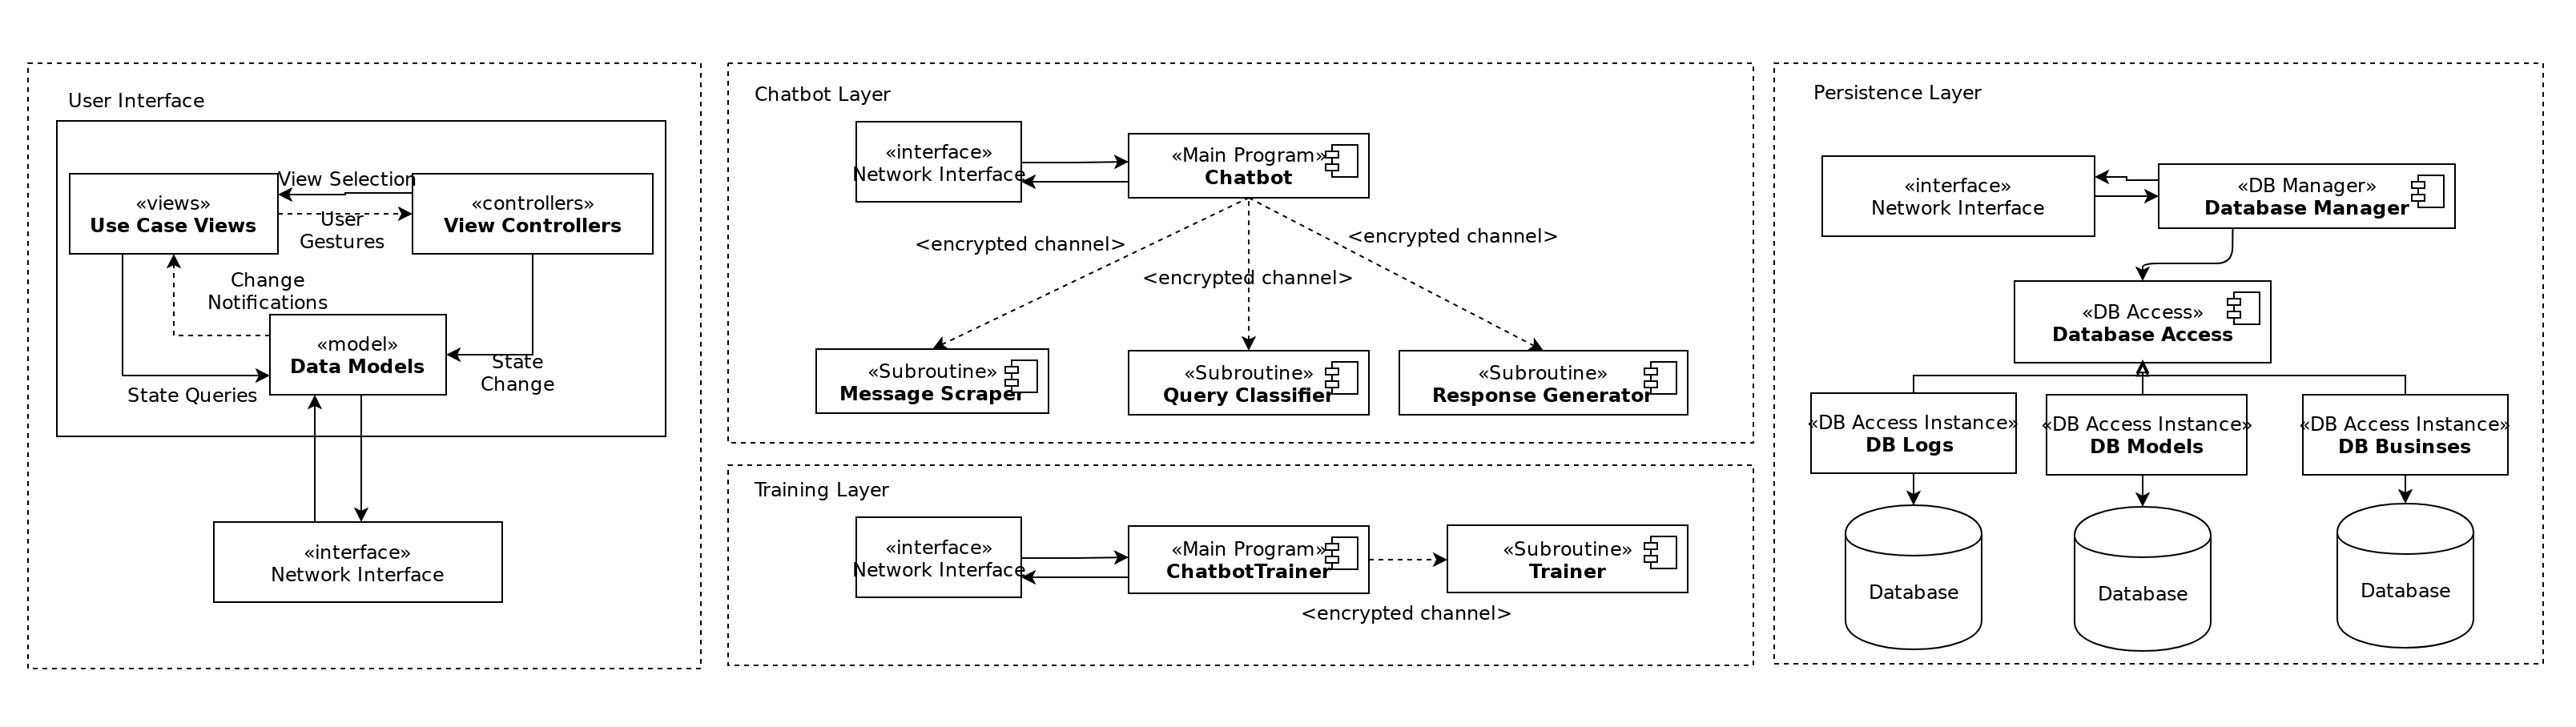
\includegraphics[width=1.25\textwidth]{../../images/Botic_Layered_Architecture.png}
	\caption{Architectural Stye of the System}
\end{figure}

The allowed-to-use relation here is denoted by the geometric adjacency of the layers from left to right-- layers on the left use layers on the right and the layers on the right are used by the layers on the left ONLY. The connections between each layer are made to be through encrypted channels. An appropriate technology will be used to implement this during the implementation phase e.g. SSL.

\paragraph{The User Interface Subsystem}
The User Interface Layer that is also an interactive subsystem uses an MVC architectural style. Using this architectural style, we ensure that user interface interface functionality, something that tends to change frequently especially in response to knew design trends *Quote IMY theory notes, be kept seperate from the application functionality and yet be ever responsive to user input, the most important thing in an interactive system\cite{Book:2}. This is the solution:

\begin{figure}[H]
	\centering
	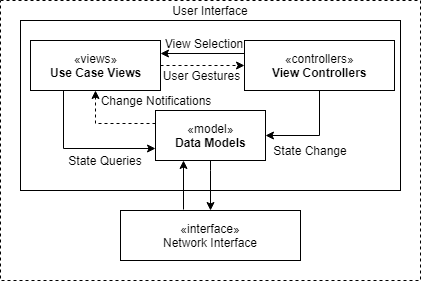
\includegraphics[width=0.5\textwidth]{../../images/User_Interface_MVC.png}
	\caption{Architectural Style of the User Interface}
\end{figure}

\paragraph{The Chatbot Layer}
The Chatbot Layer is a transformational subsystem, and will use a Main Program and Subroutines architectural style.

\begin{figure}[H]
	\centering
	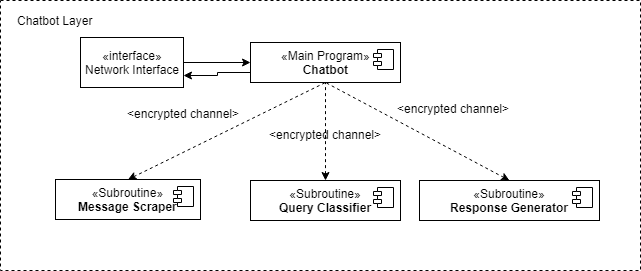
\includegraphics[width=0.8\textwidth]{../../images/Chatbot_Layer_Architecture.png}
	\caption{Architectural Style of the Chatbot Layer}
\end{figure}

\paragraph{The Training Layer}
This layer is a transformational subsystem and will also use a Main Program and Subroutines architectural style.

\begin{figure}[H]
	\centering
	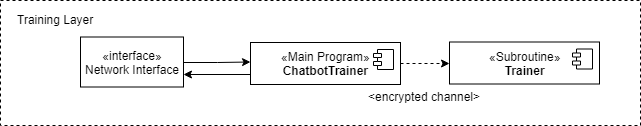
\includegraphics[width=0.8\textwidth]{../../images/Training_Layer_Architecture.png}
	\caption{Architectural Style of the Training Layer}
\end{figure}

The ChatbotTrainer is a single container that has 4 instances: these are to service requests from the user interface (requests which are sent by the Administrator user), one to train the Message Scraper, one to train the Classifier, and one to train the Response Generator. It uses the Strategy Desgin Pattern to switch different training strategies/methods to suit each subsystem it services. This results in multiple instances of the same subsystem, but each using a different training method and data on a different chatbot subsystem.

\paragraph{The Persisitance Layer}
This layer is a clear candidate for the Persistence Framework architectural style, and it's architectural style is just that. Here is our solution:

\begin{figure}[H]
	\centering
	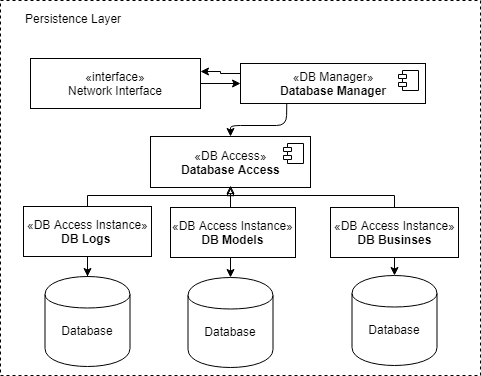
\includegraphics[width=0.6\textwidth]{../../images/Persistence_Layer_Architecture.png}
	\caption{Architectural Style of the Persistence Layer}
\end{figure}

In accordance to the architectural tactics we have chosen to observe to achieve availability and security quality attributes and requirements, in particular the security tactic to seperate access and data of different sensitivities, we have made the decision to have three databases. The first is for logs and audit trails, the second for the data models what would be used for the chatbot subsystems, and the third for recording queries and responses-- data that is concerned with the functional business processes.

\section{References}
\bibliographystyle{IEEEtran}
\bibliography{references}
%%IEEE. IEEE Std 830-1998 IEEE Recommended Practice for Software Requirements Specifications. IEEE Computer Society, 1998
%%http://www.cse.msu.edu/~chengb/RE-491/Papers/SRSExample-webapp.doc
%%TripleParity docs

\end{document}